\documentclass[12pt,a4paper,twoside]{article}
%\documentclass[a4paper,12pt]{report}
\usepackage[utf8]{inputenc} % Pacote para acentuação
\usepackage[portuguese]{babel} % Para quem vai escrever em PT-PT
\usepackage[a4paper,width=150mm,top=20mm,bottom=20mm]{geometry}
%\usepackage[lmargin=2cm,tmargin=2cm,rmargin=2cm,bmargin=2cm]{geometry}
\usepackage{indentfirst} % Identacao primeiro paragrafo
\usepackage[pdftex]{graphicx} % Pacote para inserir imagens!!!!
\usepackage{subfig} % Pacote para inserir figuras lado a lado!!
\usepackage{blindtext} % Texto aleatório


\title{Formatação de Figuras}
\author{Rafael Alves}
\date{\today}

\begin{document}

\maketitle


\section{Formatação de Imagens}
\subsection{Inserir Imagem}

\begin{figure}[!htb]   % here e top
    \centering
    \caption{Logo ISEC}
    
\includegraphics[width=13cm]{Imagens/ISEC.png}\\
    {\footnotesize Fonte: Elaborada pelo ISEC.}
    \label{fig01}
\end{figure}


\subsection{Imagens lado a lado}

\begin{figure}[!htb]
    \centering
    \caption{Exemplo de figuras lado a lado:}
    \label{figlado}
    \subfloat[DEIS \label{figdeis}]{
        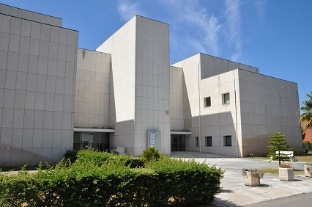
\includegraphics[width=0.30\textwidth]{Imagens/DEIS.jpeg}
    }\hfill % vai gerar um pequeno espaço entre as imagens
     \subfloat[ISEC \label{figisec}]{
        
\includegraphics[width=0.48\textwidth]{Imagens/ISEC.png}
    }
\end{figure}

Eu hoje estou a criar um documento em LaTeX sobre formatação de imagens e inseri uma figura que é a Figura \ref{figlado}.\\

\section{Inserir imagens lado a lado dentro de texto}

Lorem Ipsum is simply dummy text of the printing and typesetting industry. Lorem Ipsum has been the industry's standard dummy text ever since the 1500s, when an unknown printer took a galley of type and scrambled it to make a type specimen book.

\begin{figure}[!htb]
    \centering
    \caption{Exemplo de figuras lado a lado:}
    \label{figladoalado}
    \subfloat[DEIS \label{figdeis1}]{
        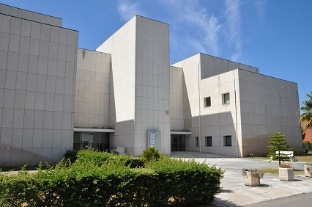
\includegraphics[width=0.30\textwidth]{Imagens/DEIS.jpeg}
    }\hfill % vai gerar um pequeno espaço entre as imagens
     \subfloat[ISEC \label{figisec1}]{
        
\includegraphics[width=0.48\textwidth]{Imagens/ISEC.png}
    }
\end{figure}

Lorem Ipsum is simply \textbf{Figura \ref{figladoalado}} dummy text of the printing and typesetting industry. Lorem Ipsum has been the industry's standard \textbf{Figura \ref{figdeis1}} dummy text ever since the 1500s, when an unknown printer took a galley of type and scrambled it to make a type specimen book. It \textbf{Figura \ref{figisec1}} has survived not only five centuries, but also the leap into electronic typesetting, remaining essentially unchanged.

\end{document}